%%%%%%%%%%%%%%%%%%%%%%%%%%%%%%%%%%%%%%%%%%%%%%%%%%%%%%%%%%%%%%%%%%%%%%%%
%                                                                      %
% LaTeX, FIIW thesis template                                          %
%                                                                      %
%%%%%%%%%%%%%%%%%%%%%%%%%%%%%%%%%%%%%%%%%%%%%%%%%%%%%%%%%%%%%%%%%%%%%%%%
% The document format below can be used for a distributable PDF or when you print single sided
\documentclass[11pt,a4paper,oneside]{book}
% If you want to print your thesis double-sided on paper, you can use the settings below
%\documentclass[11pt,a4paper]{book}

% For Campus GroepT use the two-column paper layout
%\documentclass[11pt,a4paper,twocolumn]{report}

%%% Load the FIIW template
%%% You should specify your campus : groept, denayer, gent, geel and brugge are implemented
%%% You can hide parts of the preface by specifying some option:
%%% e.g. : noacknowledgements, noabstract, nosamenvatting, nolistoffigures, nolistoftables, nolistofsymbols
\usepackage[groept]{fiiw}


%%% Load some other basic packages
\usepackage[dutch,english]{babel}
\usepackage[latin1]{inputenc}           % needed if you have special characters in your text
%\usepackage[utf8]{inputenc}            % if your text is encoded in utf8 (and not latin1) use this package

\usepackage{natbib}						% used for cites from the bib file in your text
\usepackage{listings}             		% used for displaying source code (java, c, matlab,...)
\usepackage{verbatim}					% used for inline formatting of source code, terminal commands, ...
\usepackage{hyperref}					% include hyperlinks in the resulting PDF
\usepackage{url}						% add url's with \url{http://}
\usepackage{amsmath}					% extend math features
\usepackage[final]{pdfpages}            % include pdf's e.g.: a paper or a poster
\usepackage{float}                      % adds [H] to figure env. Puts a figure where you want it e.g. \begin{figure}[H]
\usepackage{longtable}					% used for tables that strech over muliple pages
\usepackage[toc, acronyms]{glossaries}	% used by the list of symbols

% generate lorum ipsim text in template
\usepackage{lipsum}

%%% configure layout for source code listings
%\definecolor{keyword}{rgb}{0.3,0.3,0.3}
%\definecolor{string}{rgb}{0.7,0.7,0.7}
\lstset{
	language = Java,
	basicstyle=\scriptsize\ttfamily,
	numbers=left,
	numberstyle=\tiny,
	tabsize=2,
	showspaces=false,
	frame=single,
	breaklines=true,
%	keywordstyle=\bfseries\color{keyword},
%	stringstyle=\color{string},
	extendedchars=true,
	xleftmargin=0.3\linewidth,
	xrightmargin=0.1\linewidth
}

%%% abstract, acknowledgements and list of symbols are located in another file
%%% list the filenames where you created them. If you omit one of these the page
%%% is not displayed
\acknowledgementsfile{chapters/acknowledgements}	% .tex file with acknowledgements
\abstractENfile{chapters/abstract}					% .tex file with EN abstract (in English)
%\abstractNLfile{chapters/samenvatting}				% .tex file with NL abstract (in Dutch, for Dutch students only)
\listofsymbolsfile{chapters/symbols}				% .tex file with list of symbols

%%% select the main language of your document (default = dutch)
%%% (you can select a different language for the cover page below)
%\documentlanguage{dutch}
\documentlanguage{english}

%%% if the cover page needs to be a different language as the main document, this can be set
%%% if you do not specify a coverlanguage, the cover will have the same langugage as the document
%\coverlanguage{dutch}

%%% information about you, your thesis, supervisor, ...
\program{Electronics Engineering}
\title{Thesis Title}
\subtitle{Thesis Subtitle (optional)}
\firstnameA{Firstname}
\lastnameA{Lastname}
\firstnameB{Firstname2}
\lastnameB{Lastname2}
\academicyear{2021 - 2022}
% Supervisor should be from your campus
\supervisor{My Supervisor}
\supervisorEmail{My.supervisor@KULeuven.be}
% Co-supervisor can be from an external company of your campus
\cosupervisorA{My Co-supervisor}
\cosupervisorACompany{A Company, Somestreet 10, 1234 City, Belgium}
\cosupervisorAEmail{My.CoSupervisor@A-Company.be}
%\cosupervisorB{Second Co-supervisor}
%\cosupervisorBCompany{FIIW Campus GroepT, A. Vesaliusstraat 13, 3000 Leuven, Belgium}
%\cosupervisorBEmail{Second.CoSupervisor@KULeuven.be}

%%% if embargo is needed, specify the date until when it is needed
%\embargo{12-12-2030}

\begin{document}

	\preface
	\chapter{Introduction}

\lipsum[1]
\cite{Castleman98}

\section{Requirements analysis}

\lipsum[1]





	\chapter{Design/Materials}

\lipsum[1]

\begin{figure}[h]
	\centering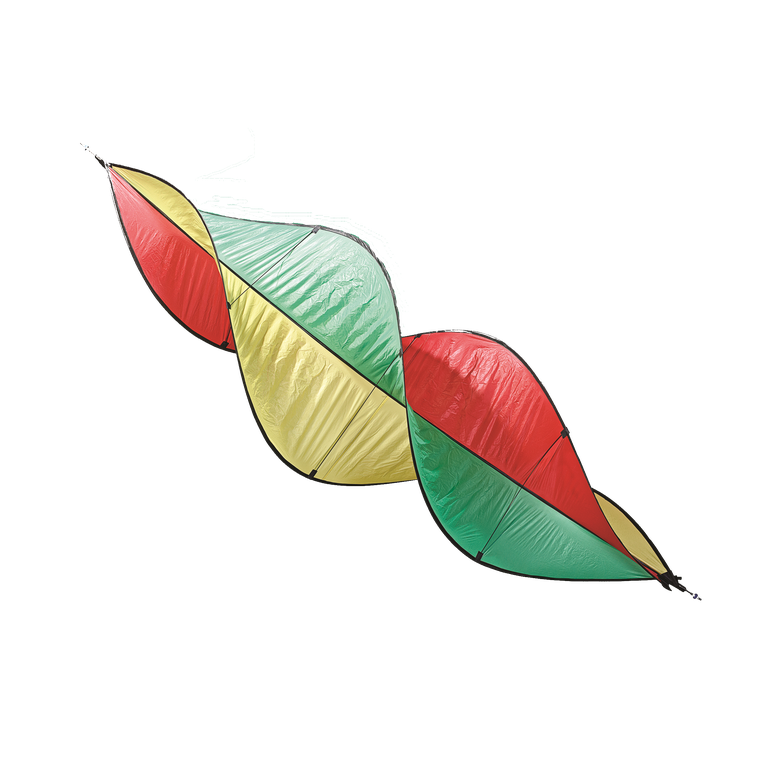
\includegraphics[height=5cm]{./images/fiiw}
	\caption{A random image}
\end{figure}

	\chapter{Implementation}
\section{Software}
Talk about the software used for developement, tools, OS. 
Give an overview of data structure for the toeplitz and vector, 
any relevant information about the buffers to store intermediate 
results. \\ Include snippets of datasplits and 
generation of nodes in tree. Talk about dependencies of 
commands and how we manage the dependencies (mention why 
there could be concurrency problems between processes). 
\\ Talk about command generation process 
\section{Hardware} 
\begin{enumerate}
	\item Talk about dispatch system 
	\item The processing pool and simd processors 
	\item Arbitrage for BW access 
\end{enumerate}







	\chapter{Evaluation}

Here we will talk about imoprtant metrics and how we can evaluate our system. \\
Important metrics could include processor utilization, scalability, bottlenecks(BW or compute) \\
Tests that we use to check accuracy/memory efficiency or resources \\
What input types did we test? \\ 
Comparision with other systems like intel's SIMD extention (maybe on a standard CPU) \\ 

	\chapter{Discussion}

\lipsum[1]
	\chapter{Conclusion}
Conclusion to paper. 

	%%% Bibliography: references. included from bibliography.bib
	%%% Only referenced items are displayed in the final document
	%\nocite{*}			% if you also want to display the unreferenced items in your bibliografy uncomment this
	\bibliographystyle{apalike}
	\bibliography{bibliography}

	%%% appendices
    \appendix
    \appendixpage
	% when you are using the twocolumn layout for your thesis appendixes may/can be in a 'singlecolumnsection'
\begin{singlecolumnsection}
\chapter{Some extra info}

\lipsum[1]

\end{singlecolumnsection}

	%%% Apendix from other pdf
%	\chapter{Poster}
%	\includepdf{poster.pdf}

	\backcover
\end{document}
